\documentclass[titlepage, a4paper, 12pt]{article}
\usepackage[swedish]{babel}
\usepackage[utf8]{inputenc}
\usepackage{verbatim}
\usepackage{fancyhdr}
\usepackage{graphicx}
\usepackage{parskip}
\usepackage{comment}
\usepackage{varioref}

% SourceCode
\usepackage{listings}
\usepackage{color}

% Include pdf with multiple pages ex \includepdf[pages=-, nup=2x2]{filename.pdf}
\usepackage[final]{pdfpages}
% Place figures where they should be
\usepackage{float}

% SourceCode
\definecolor{keywordcolor}{rgb}{0.5,0,0.75}
\lstset{
  inputencoding=utf8,
  language=Java,
  extendedchars=true,
  basicstyle=\scriptsize\ttfamily,
  stringstyle=\color{blue},
  commentstyle=\color{red},
  numbers=left,
  firstnumber=auto,
  numberblanklines=true,
  stepnumber=1,
  showstringspaces=false,
  keywordstyle=\color{keywordcolor}
  % identifierstyle=\color{identifiercolor}
}

% Float for text
\floatstyle{ruled}
\newfloat{kod}{H}{lop}
\floatname{kod}{Kodsnutt}

% vars
\def\title{Genetiska algoritmer}
\def\preTitle{Laboration 3}
\def\kurs{Emergenta system, VT-09}

\def\namn{Andreas Jakobsson}
\def\mail{dit06ajs@cs.umu.se}
\def\namnTva{Anton Johansson}
\def\mailTva{dit06ajn@cs.umu.se}

\def\pathtocode{$\sim$dit06ajn/edu/emergenta-system/lab3/src}

\def\handledareEtt{Jonny Pettersson, jonny@cs.umu.se}
\def\handledareTva{Anders Broberg, bopspe@cs.umu.se}

\def\inst{datavetenskap}
\def\dokumentTyp{Laborationsrapport}

\begin{document}
\begin{titlepage}
  \thispagestyle{empty}
  \begin{small}
    \begin{tabular}{@{}p{\textwidth}@{}}
      UMEÅ UNIVERSITET \hfill \today \\
      Institutionen för \inst \\
      \dokumentTyp \\
    \end{tabular}
  \end{small}
  \vspace{10mm}
  \begin{center}
    \LARGE{\preTitle} \\
    \huge{\textbf{\kurs}} \\
    \vspace{10mm}
    \LARGE{\title} \\
    \vspace{15mm}
    \begin{large}
      \namn, \mail \\
      \namnTva, \mailTva\\
      \texttt{\pathtocode}
    \end{large}
    \vfill
    \large{\textbf{Handledare}}\\
    \mbox{\large{\handledareEtt}}
    \mbox{\large{\handledareTva}}
  \end{center}
\end{titlepage}

\newpage
\mbox{}
\vspace{70mm}
\begin{center}
% Dedication goes here
\end{center}
\thispagestyle{empty}
\newpage

\pagestyle{fancy}
\rhead{\today}
\lhead{\footnotesize{\namn, \mail\\\namnTva, \mailTva}}
\chead{}
\lfoot{}
\cfoot{}
\rfoot{}

\cleardoublepage
\newpage
\tableofcontents
\cleardoublepage

% \fancyfoot[LE,RO]{\thepage}
\cfoot{\thepage}
\pagenumbering{arabic}

\section{Problemspecifikation}\label{sec:problemspecifikation}
Laborationen gick ut på att göra ändringar i en befintlig
NetLogo\footnote{http://ccl.northwestern.edu/netlogo/} modell,
''Simple Genetic Algorithm'', som implementerar en enkel genetisk
algoritm. I modellen avgörs vilka individer som får fortplanta sig till
nästa generation med hjälp av en metod som kallas \textit{Tournament
  Selction}. Metoden fungerar genom att slumpmässigt dra tre individer
ur en population, individen med högst \textit{fitness}–värde väljes ut
för fortplantning. En individs \textit{fitness}–värde ska representera
hur pass välanpassad individen är för att lösa ett specifikt problem.

I given modell består problem som ska lösas av att individerna ska
söka efter en sträng av enbart ettor, exempel \verb!"11111"!,
\textit{fitness}–värdet är då antalet ettor i en individs sträng.

Uppgifter som ska lösas (från originalspecifikation):
\begin{itemize}
\item Implementera ytterligare två olika valfira varianter av
  selektion (implementation enligt An Introduction to Genetic
  Algorithms, Melanie Mitchell).
\item Jämför de tre varianterna av selektion med avseende på hur bra
  de bidrar till att så fort som möjligt hitta lösningen
\item Presentera och argumentera för det ni kommer fram till.
\item Reflektera kring laborationen och genetiska algoritmer.
\end{itemize}

% Att göra
% Två valfira varianter av selektion:
% - Tournament selection är implementerad
% - Fitness-Proportionate Selection / Roulette Wheel Selection and Stochastic
%   Universal Sampling
%      reproduce nr of times = individual fitness / mean(population
%      fitness). Dvs de som har bra fittness får fortplanta sig mer än
%      de andra.

\subsection{Frågor som ska behandlas}
I problemspecifikationen finns följande frågor som denna rapport ska
behandla.

\begin{itemize}
\item Vilken selektionsmetod passar bäst för problemet i modellen och varför?
\item För vilken typ av problem passar respektive selektionsmetod?
\item Vilka applikationsområden kan du se för evolutionära algoritmer?
\item För vilken typ av problem ser ni att evolutionära algoritmer
  kommer till mest nytta?
\item Försöka också att sätta in laborationen i ett större sammanhang. 
\end{itemize}
Laborationsspecifikation finns i original på sidan:\\
\verb!http://www.cs.umu.se/kurser/5DV017/VT09/lab/lab3.html!

\section{Användarhandledning}
Källkoden till implementationen lab3.nlogo som diskuteras i denna
rapport finns att hitta på:

\verb!~dit06ajn/edu/emergenta-system/lab3/src!

Öppna filen i NetLogo för att köra den.

\subsection{Förklaring av användargränssnittet}
Nedan följer en förklaring av de knappar och reglage som förekommer i
användargränssnittet:

\begin{itemize}
\item \textbf{population-size} - antalet individer i uppsättningen.
\item \textbf{crossover-rate} - antal procent av populationen som ska användas för sexuell reproduktion.
\item \textbf{mutation-rate} - antal procent av individer som kan muteras.
\item \textbf{go} - denna knapp sätter igång förloppet. Metoden upprepas tills dess att målet är uppfyllt (enbart ettor, enbart vita sträck). Setup måste köras en gång innan denna knapp får användas.
\item \textbf{setup} - initierar parametrar till simuleringen.
\item \textbf{step} - anropar proceduren go endast en gång.
\item \textbf{selection-method} - anger vilken selektionsmetod som ska användas.
\item \textbf{Run test script} - startar det hårdkodade testskriptet
  och sparar data till mappen \textit{data}.
\end{itemize}

För information om funktioner från den omodifierade NetLogo–modellen
se fliken \textit{Information} i NetLogo.

\section{Algoritmbeskrivning}
Nedan följer förklaring över de selektionsmetoder som är
implementerade i denna laboration. Alla selektionsmetoder
implementerades utifrån beskrivningar givna i boken \textit{An
  introduction to genetic algorithms}, \cite{gen-intro}.

\subsection{Roulette Wheel}\label{sec:roulette-wheel}
Selektionsalgoritmen \textit{Roulette Wheel} har fått sitt namn på
grund av att metoden kan liknas vid att snurra ett Roulette–hjul där
vissa individer har större sannolikhet att väljas baserat på dess
\textit{fitness}.

För algoritmen räknas ett värde, \textit{expected-value}, som ger en
fingervisning om hur välanpassad en individ är gentemot de andra
individerna i populationen. Detta värde räknas ut för varje individ
genom att dela dess \textit{fitness}–värde med medelvärdet av hela
populationens \textit{fitness}–värden.

Följande metod följdes för att välja individer för sexuell
reproduktion:

\begin{enumerate}
\item Summera totala antalet individer i populationen, kalla denna
  summa \textit{T}.
\item Upprepa följande steg antalet gånger som ett urval ska göras. I
  denna laboration bestäms detta av parametern
  \textit{crossover-rate}.
  \begin{itemize}
  \item Välj ett slumpmässig tal \textit{r} mellan 0 och
    \textit{T}. Iterera över individerna i populationen, summera
    värdet på \textit{expected-value} tills summan är större än eller
    lika med \textit{r}. Välj ut individen vars värde går över denna gräns.
  \end{itemize}
\end{enumerate}

\subsection{Roulette Wheel with Sigma Scaling}
Selektionsmetoden \textit{Roulette Wheel with Sigma Scaling} används
exakt som \textit{Roulette Wheel}, se avsnitt
\ref{sec:roulette-wheel}, förutom att individernas
\textit{expected-value} räknas ut enligt följande formel, (direkt
tagen ur \cite{gen-intro}):

\begin{displaymath}
  \textrm{ExpVal(i,t)} = \left\{ \begin{array}{ll}
      1 + \frac{f(i) - \overline{f}(t)}{2\sigma(t)} & \textrm{om } \sigma(t) \neq 0 \\
      1.0 & \textrm{om } \sigma(t) = 0
    \end{array} \right.
\end{displaymath}
  
Här avser $f(i)$ \textit{fittness} för individ $i$, $\overline{f}(t)$
avser medelvärdet för populationens \textit{fitness}–värde vid tiden
$t$ och $\sigma(t)$ är standardavvikelsen vid tiden $t$. Anledning
till denna ändring i \textit{expected-value} är att försöka variera
vikten av individers \textit{fitness} så att en skillnaden på
\textit{expected-value} ökar i slutet av en körning när det typsikt är
mindre skillnad bland individernas \textit{fitness}. Detta ska
förhindra för tidig konvergens.
% TODO: forsätt i diskussion ey.

\subsection{Steady State}
% TODO piece of cake
Selektionsmetoden \textit{Steady State} är implementerad så att enbart
en tredjedel av de bästa individerna i varje generation har möjlighet
till sexuell reproduktion. Två tredjedelar av individerna med bäst
\textit{fitness} överlever utan förändring. På alla överlevande utförs
mutation med sannlikhet bestämd av parametern
\textit{mutation-rate}. En tredjedel av de sämst anpassade individerna
dör ut. Procedurerna för selektion visas i kodsnutt nedan.

\begin{kod}[H]
  \begin{scriptsize}
\begin{verbatim}
to-report steady-state-selection
   report one-of (max-n-of (count old-generation / 3) old-generation [fitness])
end

to-report steady-state-survivor
   report one-of (max-n-of (count old-generation *  (2 / 3)) old-generation [fitness])
end
\end{verbatim}
  \end{scriptsize}
\end{kod}

\section{Metod för testning}
De implementerade selektionsmetoderna utvärderas genom att jämföra
antalet omgångar, hädan efter kallade ticks, det tar för metoden att
hitta en fullständig lösning. För att generera testdata gjordes ett
\textit{test-script} som kan aktiveras från
användargränssnittet. Test-scriptet sätter programmets parametrar och
itererar varje selektionsmetod ett förinställt antal gånger. Antalet
ticks som krävs för att hitta en lösning sparas i en textfil. Efter
att en sorts selektionsmetod har körts klart avslutas filen med
medelvärdet och standardavvikelsen för den insamlade datan. Därefter
startar en ny fil där data från nästa selektionsmetod sparas. När alla
valda selektionsmetoder har kört klart avslutas
skriptet. Sammanställning av resultaten kan ses under avsnitt
\ref{sec:resultat}. Vi testade samma parameterinställningar och gjorde
olika antal körningar för att se hur många som krävdes för att få fram
ett stabilt medelvärde med en liten standardavvikelse. Resultatet av
detta vara att det räckte med tio körningar eftersom värdena blev
mycket nära de som ficks efter hundra körningar. Jämför bilaga
\ref{Tournament-100-70-0.5.dat} med
\ref{Tournament100runsedited.dat}. För att testa de olika
parametrarnas inverkan på resultatet varierades dessa mellan olika
värden, se avsnitt \vref{sec:resultat} för diskussion kring valda
värden.

\section{Resultat}\label{sec:resultat}
% Tabell och sådant
Följande tabeller redovisar antalet generationer det behövdes i medel
för att hitta optimal lösning på givet problem med olika
parameterinställningar och olika selektionsmetoder. För varje
parameterinställning gjordes tio körningar och därefter räknades
medelvärde och standardavvikelse ut.

För att göra körningarna konsekventa valdes \textit{crossover-rate}
till 70 \%, ett godtyckligt tal. För att testa populationsstorlekens
inverkan testades körningar med 100 och 200 individer i varje
population, också dessa tal är godtyckligt valda. Eftersom
förhållandena mellan de olika selektionsmetoderna bibehölls vid båda
värdena gjordes ej ytterligare variationer av
populations\-storlek. Mutationens inverkan testades genom att
körningar gjordes med \textit{mutation-rate} satt till 0.5 \%, 1 \%
och 2 \%, tre godtyckliga tal. Vid 2 \% var standardavvikelsen så pass
hög att vidare ökning av \textit{mutation-rate} kändes irrelevant.

\begin{figure}[H]
\begin{tabular}{lccc}
% BEGIN RECEIVE ORGTBL mutation
\hline
100-70-0.5 & Roulette Wheel Sigma & Steady State & Tournament \\
\hline
Medelvärde & 42.2 & 41.4 & 44 \\
Standardavvikelse & 2.8 & 3.5 & 5.7 \\
\hline
% END RECEIVE ORGTBL mutation
\end{tabular}
\caption{Population: 100, Crossover-rate: 70, Mutation: 0.5}\label{tab:mut05}
\end{figure}
\begin{comment}
#+ORGTBL: SEND mutation orgtbl-to-latex :splice t :skip 0
|-------------------+----------------------+--------------+------------|
| 100-70-0.5        | Roulette Wheel Sigma | Steady State | Tournament |
|-------------------+----------------------+--------------+------------|
| Medelvärde        |                 42.2 |         41.4 |         44 |
| Standardavvikelse |                  2.8 |          3.5 |        5.7 |
|-------------------+----------------------+--------------+------------|
\end{comment}

\begin{figure}[H]
\begin{tabular}{lccc}
% BEGIN RECEIVE ORGTBL population
\hline
200-70-0.5 & Roulette Wheel Sigma & Steady State & Tournament \\
\hline
Medelvärde & 33.5 & 33.2 & 35.2 \\
Standardavvikelse & 2.6 & 2.2 & 2.7 \\
\hline
% END RECEIVE ORGTBL population
\end{tabular}
\caption{Population: 200, Crossover-rate: 70, Mutation: 0.5}\label{tab:pop200}
\end{figure}
\begin{comment}
#+ORGTBL: SEND population orgtbl-to-latex :splice t :skip 0
|-------------------+----------------------+--------------+------------|
| 200-70-0.5        | Roulette Wheel Sigma | Steady State | Tournament |
|-------------------+----------------------+--------------+------------|
| Medelvärde        |                 33.5 |         33.2 |       35.2 |
| Standardavvikelse |                  2.6 |          2.2 |        2.7 |
|-------------------+----------------------+--------------+------------|
\end{comment}

\begin{figure}[H]
\begin{tabular}{lccc}
% BEGIN RECEIVE ORGTBL mutationone
\hline
100-70-1 & Roulette Wheel Sigma & Steady State & Tournament \\
\hline
Medelvärde & 43 & 42.45 & 46.9 \\
Standardavvikelse & 6.4 & 4.8 & 4.0 \\
\hline
% END RECEIVE ORGTBL mutationone
\end{tabular}
\caption{Population: 100, Crossover-rate: 70, Mutation: 1}\label{tab:mut1}
\end{figure}
\begin{comment}
#+ORGTBL: SEND mutationone orgtbl-to-latex :splice t :skip 0
|-------------------+----------------------+--------------+------------|
| 100-70-1          | Roulette Wheel Sigma | Steady State | Tournament |
|-------------------+----------------------+--------------+------------|
| Medelvärde        |                   43 |        42.45 |       46.9 |
| Standardavvikelse |                  6.4 |          4.8 |        4.0 |
|-------------------+----------------------+--------------+------------|
\end{comment}

\begin{figure}[H]
\begin{tabular}{lccc}
% BEGIN RECEIVE ORGTBL mutationtwo
\hline
100-70-2 & Roulette Wheel Sigma & Steady State & Tournament \\
\hline
Medelvärde & 277.35 & 309.15 & 462.95 \\
Standardavvikelse & 278.6 & 220.6 & 287.3 \\
\hline
% END RECEIVE ORGTBL mutationtwo
\end{tabular}
\caption{Population: 100, Crossover-rate: 70, Mutation: 2}\label{tab:mut2}
\end{figure}
\begin{comment}
#+ORGTBL: SEND mutationtwo orgtbl-to-latex :splice t :skip 0
|-------------------+----------------------+--------------+------------|
| 100-70-2          | Roulette Wheel Sigma | Steady State | Tournament |
|-------------------+----------------------+--------------+------------|
| Medelvärde        |               277.35 |       309.15 |     462.95 |
| Standardavvikelse |                278.6 |        220.6 |      287.3 |
|-------------------+----------------------+--------------+------------|
\end{comment}

Komplett data finns i bilaga
\ref{Roulette-Wheel-Sigma-100-70-0.5.dat}–\ref{Tournament-200-70-0.5.dat}.

\section{Reflektioner}\label{sec:reflektioner}
Nedan avsnitt beskriver reflektioner som gjorts med avseende på
frågorna från problemspecifikationen.

\subsection{Mutation}
Vid testen där mutationen varierades mellan 0.5–2 syns en markant
skillnad i konvergeringstid när mutationsnivån var på 2, se tabell i
figur \ref{tab:mut2}. Anledning till denna drastiska ökning var att
populationen fastnade i en suboptimal lösning. Anledningen till den
stora standardavvikelsen är att denna subotimala lösning låg mycket
nära den optimala och slumpen inblandad vid mutation var avgörande för
att lösningen skulle ändras från suboptimal till optimal, se figur
\ref{fig:images/Roulette-Wheel-Sigma-100-70-2-20}.

\begin{figure}[H]
  \begin{center}
    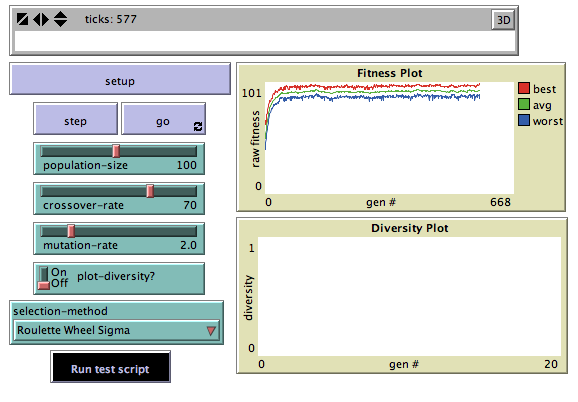
\includegraphics[width=110mm]{images/Roulette-Wheel-Sigma-100-70-2-20.png}
    \caption{Mutation: 2.0}
    \label{fig:images/Roulette-Wheel-Sigma-100-70-2-20}
  \end{center}
\end{figure}

\subsection{Övriga reflektioner}
% Vilken selektionsmetod passar bäst för problemet i modellen och
% varför?
Eftersom resultatet inte pekar på större skillnader i tidsåtgång är
det svårt att resonera om skillnader mellan prestandan av
selektionsmetoderna som löste uppgiften. Den redan implementerade
Tournament-metoden står ändå ut med tanke på den enkla
implementationen och kan därför ses som en segrare. Ett förslag till
förbättring till denna metod vore att lägga till så kallad
Elitism-procedur \cite{gen-intro} för att låta en del av de bästa
individerna gå vidare direkt till nästa generation och alltså
eliminera risken av att de blir undansparkade av slumpen.
    
% För vilken typ av problem passar respektive selektionsmetod?
Med avseende på tidsåtgång förlorar Roulette Wheel som sällan hittade
rätt lösning. Problemet var att utvecklingen av populationen
avstannade (premature konvergence) eftersom variansen blev för liten
och de med bättre fitness tappade övertaget. Denna selektionsmetod
lämpar sig alltså bara inledningsvis i evolutionen eller om ett
perfekt resultat inte är nödvändigt. Se diagrammet \textit{Fitness Plot} i
figur \ref{fig:images/premature-convergence} på ett exempel för hur
detta kan se ut.

\begin{figure}[H]
  \begin{center}
    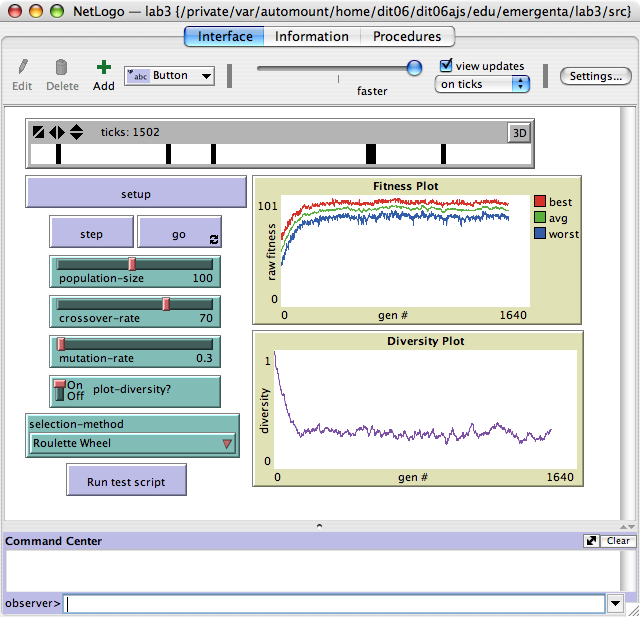
\includegraphics[width=110mm]{images/premature-convergence.png}
    \caption{För tidig konvergens, 1502 generationer}
    \label{fig:images/premature-convergence}
  \end{center}
\end{figure}

% Vilka applikationsområden kan du se för evolutionära algoritmer?
Applikationsområden för evolutionära algoritmer skulle kunna tänkas
vara problem där lösningsrymden är så pass stor att det är svår att
tänka sig fram till en lösning.

% För vilken typ av problem ser ni att evolutionära algoritmer kommer
% till mest nytta?
I laboration 1 där termiter skulle flytta träbitar till en enda hög
fanns en del parametrar att skruva på. Det fanns även flera önskvärda
beteenden som skulle uppnås. Förutom att alla träbitar skulle ligga
samlat ska de även forma en cirkulär samling. Dessutom konvergerar
högen snabbare om två konkurrerande myrsorter bygger sina högar
åtskiljt. Om en uppsättning parametrar uppfyller dessa krav kan
lösningen anses fullständig, alltså en sträng med ettor. Denna
parameterskruvning skulle kunna göras med hjälp av evolutionära
algoritmer.

Evolutionära algoritmer borde passa bra till just parameterskruvning
eftersom rätt kombination av parametrarna ej behöver vara trivial och
behöver testas fram och utvärderas.

\subsection{Slutsats}
Vi ser att \textit{Steady State}–selektionsmetoden hittar optimal
lösning snabbast i flest testfall, se avsnitt \ref{sec:resultat}.  Med
tanke på den minimala skillnaden och storleken på att
standardavvikelsen kan vi inte dra några slutsatser om vilken metod
som är snabbast. Fler test med variande parametrar skulle vara
intressant att genomföra.

\bibliographystyle{alpha}
\bibliography{books}

\newpage
\appendix
\pagenumbering{roman}
\section{Källkod}\label{sec:kallkod}
Härefter följer utskrifter från källkoden och andra filer som hör till
denna laboration

\subsection{Roulette-Wheel-Sigma-100-70-0.5.dat}\label{Roulette-Wheel-Sigma-100-70-0.5.dat}
\begin{footnotesize}
  \verbatiminput{../src/data/100-70-0.5/Roulette-Wheel-Sigma-100-70-0.5.dat}
\end{footnotesize}

\subsection{Steady-State-100-70-0.5.dat}\label{Steady-State-100-70-0.5.dat}
\begin{footnotesize}
  \verbatiminput{../src/data/100-70-0.5/Steady-State-100-70-0.5.dat}
\end{footnotesize}

\subsection{Tournament-100-70-0.5.dat}\label{Tournament-100-70-0.5.dat}
\begin{footnotesize}
  \verbatiminput{../src/data/100-70-0.5/Tournament-100-70-0.5.dat}
\end{footnotesize}


\subsection{Roulette-Wheel-Sigma-100-70-1.dat}\label{Roulette-Wheel-Sigma-100-70-1.dat}
\begin{footnotesize}
  \verbatiminput{../src/data/100-70-1/Roulette-Wheel-Sigma-100-70-1.dat}
\end{footnotesize}

\subsection{Steady-State-100-70-1.dat}\label{Steady-State-100-70-1.dat}
\begin{footnotesize}
  \verbatiminput{../src/data/100-70-1/Steady-State-100-70-1.dat}
\end{footnotesize}

\subsection{Tournament-100-70-1.dat}\label{Tournament-100-70-1.dat}
\begin{footnotesize}
  \verbatiminput{../src/data/100-70-1/Tournament-100-70-1.dat}
\end{footnotesize}

\subsection{Roulette-Wheel-Sigma-100-70-2.dat}\label{Roulette-Wheel-Sigma-100-70-2.dat}
\begin{footnotesize}
  \verbatiminput{../src/data/100-70-2/Roulette-Wheel-Sigma-100-70-2.dat}
\end{footnotesize}

\subsection{Steady-State-100-70-2.dat}\label{Steady-State-100-70-2.dat}
\begin{footnotesize}
  \verbatiminput{../src/data/100-70-2/Steady-State-100-70-2.dat}
\end{footnotesize}

\subsection{Tournament-100-70-2.dat}\label{Tournament-100-70-2.dat}
\begin{footnotesize}
  \verbatiminput{../src/data/100-70-2/Tournament-100-70-2.dat}
\end{footnotesize}

\subsection{Roulette-Wheel-Sigma-200-70-0.5.dat}\label{Roulette-Wheel-Sigma-200-70-0.5.dat}
\begin{footnotesize}
  \verbatiminput{../src/data/200-70-0.5/Roulette-Wheel-Sigma-200-70-0.5.dat}
\end{footnotesize}

\subsection{Steady-State-200-70-0.5.dat}\label{Steady-State-200-70-0.5.dat}
\begin{footnotesize}
  \verbatiminput{../src/data/200-70-0.5/Steady-State-200-70-0.5.dat}
\end{footnotesize}

\subsection{Tournament-200-70-0.5.dat}\label{Tournament-200-70-0.5.dat}
\begin{footnotesize}
  \verbatiminput{../src/data/200-70-0.5/Tournament-200-70-0.5.dat}
\end{footnotesize}

\subsection{Tournament100runsedited.dat}\label{Tournament100runsedited.dat}
\begin{footnotesize}
  \verbatiminput{../src/data/Tournament100runsedited.dat}
\end{footnotesize}

\subsection{lab3.nlogo}\label{app:lab3.nlogo}
\begin{footnotesize}
  \verbatiminput{../src/lab3.nlogo}
\end{footnotesize}
\end{document}
